\chapter{Hauptteil}
\label{sec:hauptteil}

Hier werden die zur Lösung der gestellten Aufgaben erforderlichen Arbeiten ausführlich beschrieben.
Je nach Aufgabenstellung sind benutzte Theorien und Rechenmethoden zu erläutern, 
Versuchseinrichtungen zu beschreiben, Festigkeitsnachweise zu führen, Konstruktionsbeschreibungen anzufertigen usw.
Der Text soll es dem Leser ermöglichen, die Arbeit inhaltlich zu verstehen, ohne zusätzliche Spezialliteratur 
zu benötigen, wobei davon ausgegangen wird, dass der Leser einen Bachelor-Abschluss mit einigen Grundlagenkenntnissen 
zur Luft- und Raumfahrt besitzt. Allgemein zugänglicher bzw. bekannter Lehrbuch- oder Vorlesungsstoff soll daher nicht
ausführlich wiederholt, sondern nur, soweit zum Verständnis unbedingt nötig, kurz zusammengefasst und zitiert werden. 

Es ist darauf zu achten, dass theoretische Herleitungen schlüssig sind (kontrollieren, ob jede Größe
eindeutig definiert ist; keine Gedankensprünge). Theoretische Herleitungen mit allgemeinen Bezeichnungen. 
Zahlenwerte erst im Ergebnisteil. Die im Rahmen der Arbeit gefundenen Ergebnisse sind in \kap{sec:ergebnisse} ausführlich zu diskutieren. 
Evtl. auftretende Abweichungen zwischen Theorie und Messung bzw. zwischen verschiedenen Rechenverfahren
sind zu deuten. Besonderes Gewicht ist auf die physikalische Interpretation mathematischer bzw. experimenteller 
Ergebnisse zu legen. Computerprogramme sind bezüglich ihrer Ein- und Ausgabedateien sorgfältig zu dokumentieren.
Unterroutinen sollen mit Zweck und Ein- und Ausgabeparametern dokumentiert werden. 
Ein Struktogramm, das den logischen Programmablauf darstellt, ist zu empfehlen. Der Quellcode der entwickelten 
Computerprogramme ist in einem textuellen Dateiformat (ASCII) zusammen mit der Arbeit einzureichen. 

Für den Hauptteil sind weiterhin folgende Punkte zu beachten:
\begin{itemize}
 \item Eigennamen sollen in Großbuchstaben geschrieben werden, z. B. EULER-Winkel.
Verweise auf Bilder und Tabellen sind entsprechend dieser Vorlage zu erstellen, z.B.: \abb{fig:beispiel}, \tab{tab:beispiel}.
 \item Der Raum für Text und Bilder soll möglichst gut ausgenutzt werden, so soll nicht etwa eine Seite nur eine Abbildung in der Mitte enthalten und oben und 
unten große Leerräume bleiben.
 \item Nur neue Kapitel (Einleitung, Theoretische Grundlagen, etc.) beginnen auf neuen Seiten.
 \item Formeln werden automatisch nummeriert, ein Verweis ist folgendermaßen möglich: \glg{eq:beispiel}
 \item Zu jeder Abbildung und jeder Tabelle gehört eine Bildunterschrift (Abbildung) bzw. -überschrift (Tabelle).
 \item In Abbildungen sollen die Achsen mit der entsprechenden Größe und der Dimension bezeichnet werden.
 \item Zahlen entsprechend der ISO-31 mit Tausender-Trennzeichen (Leerzeichen) schreiben: $10\;000$ und nicht $10000$
\end{itemize}

\begin{figure}[h]
 \centering
 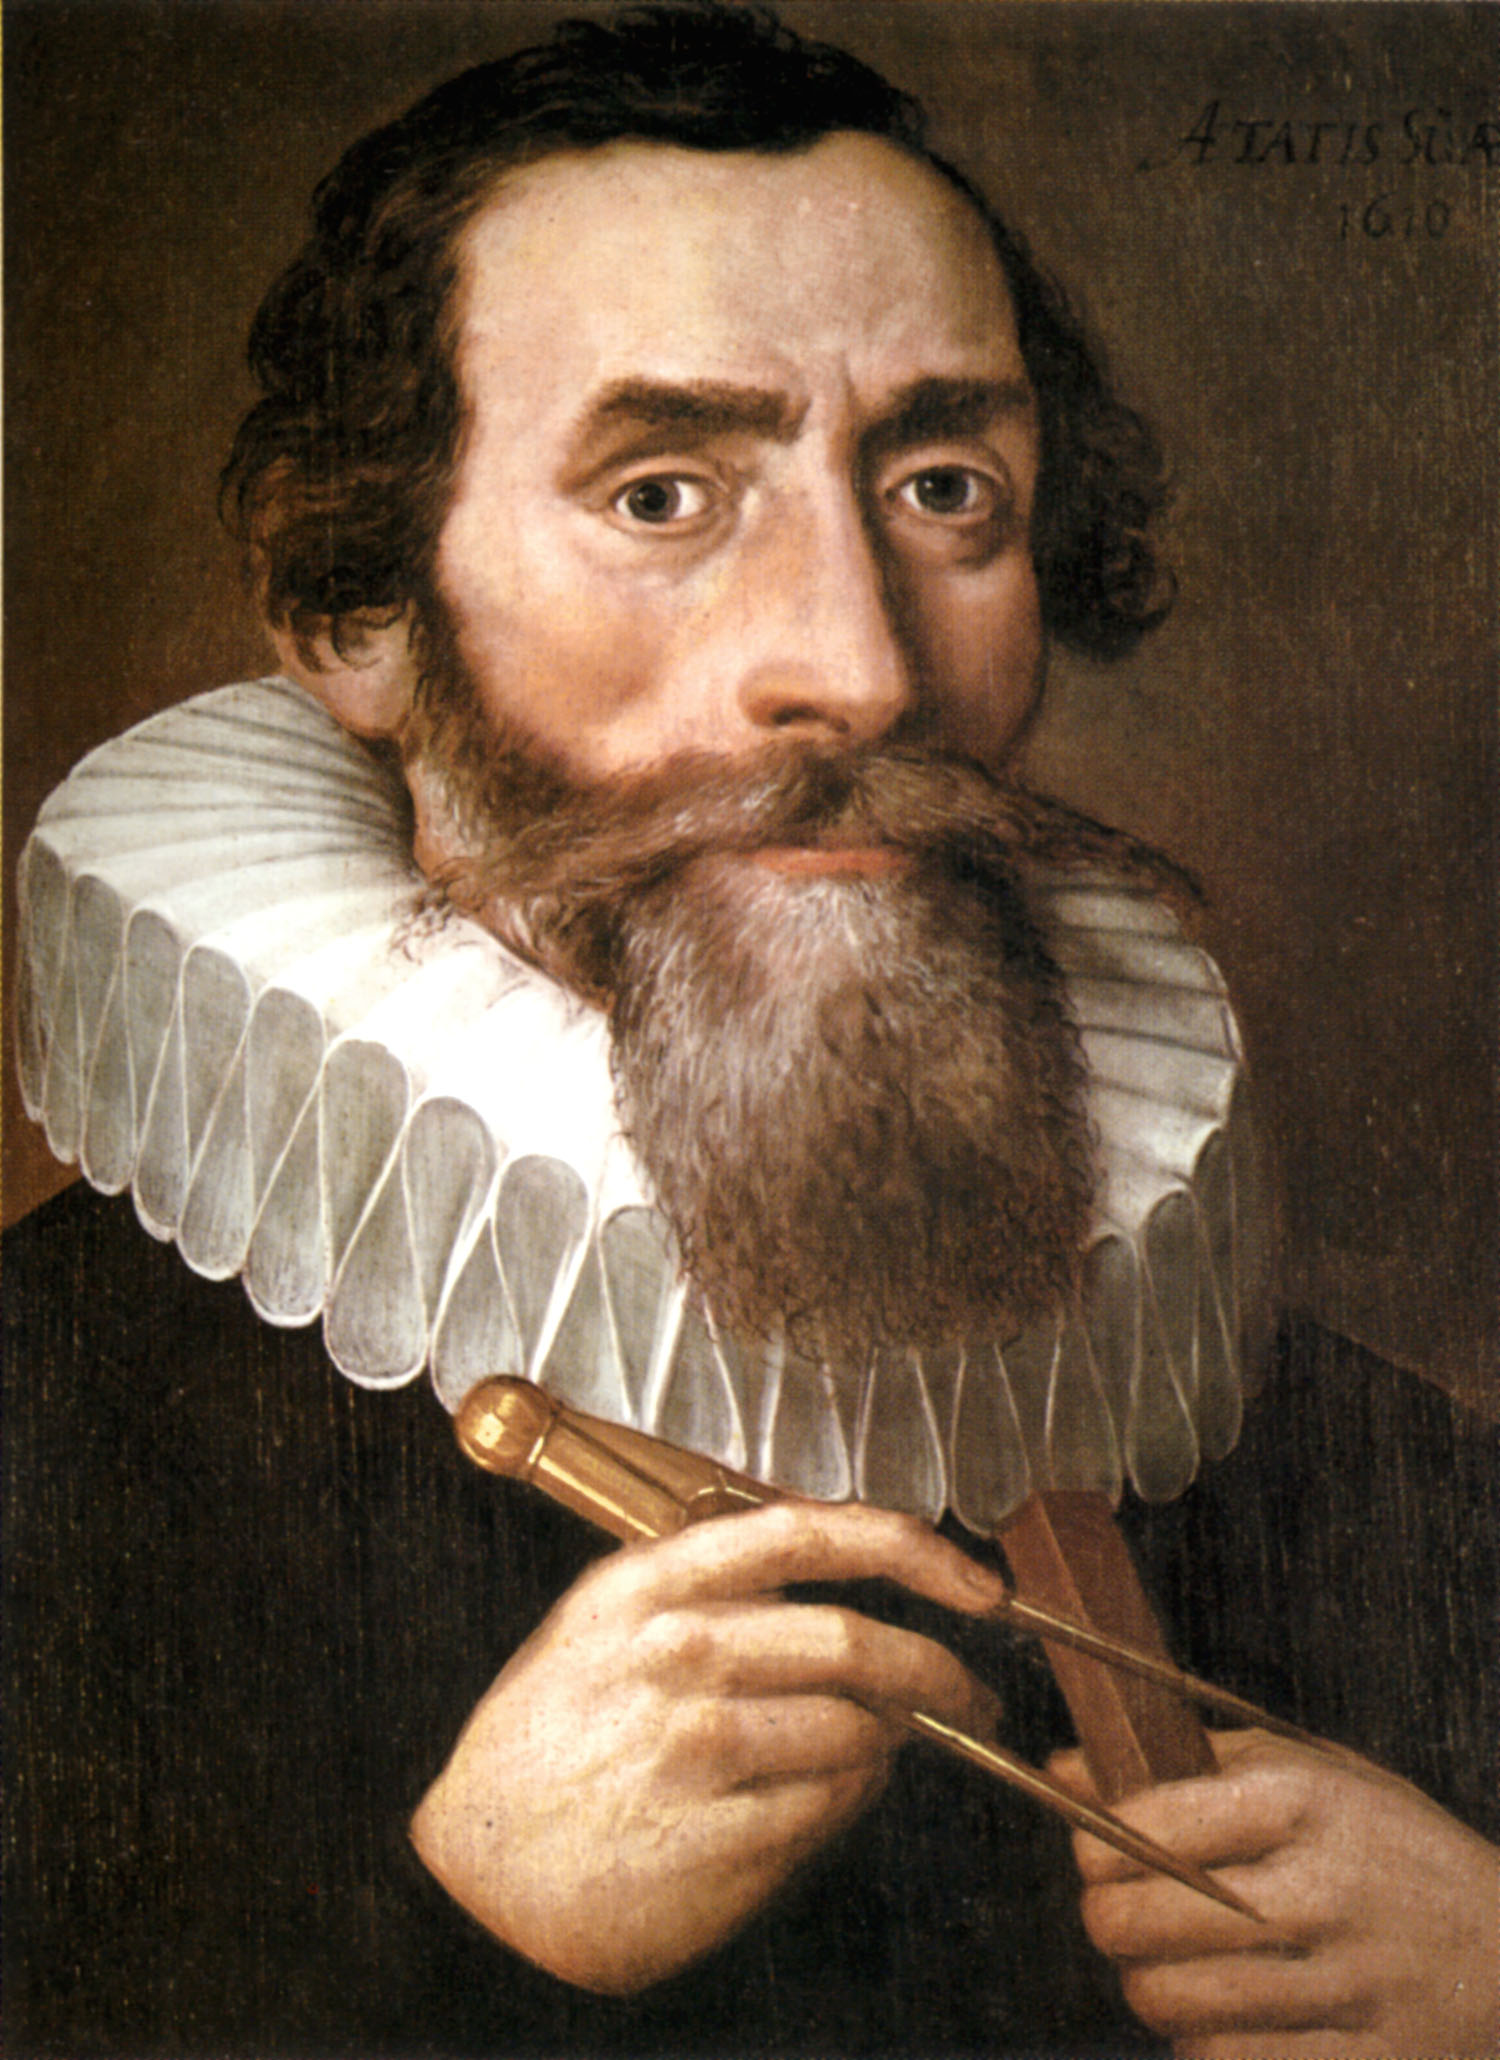
\includegraphics[width=0.3\textwidth]{kepler.jpg}
 \caption{Ein Bild von Kepler.\label{fig:beispiel}}
\end{figure}

In Tabellen ist darauf zu achten, dass möglichst wenig vertikale Striche verwendet werden, wie im Beispiel in \tab{tab:beispiel} gezeigt.
\begin{table}[h]
 \centering
 \caption{Bahntypen als Funktion der Exzentrizit\"at.\label{tab:beispiel}}
 \begin{tabular}{cl}
  \tb{Wert der Exzentrizit\"at} & \multicolumn{1}{c}{\tb{Bahntyp}} \\
  \hline
  \hline
  $\epsilon = 0$ & Kreis \\
  $0 < \epsilon < 1$ & Ellipse \\
  $\epsilon = 1$ & Parabel \\
  $\epsilon > 1$ & Hyperbel \\
  \hline
 \end{tabular}
\end{table}

\section{Referenzieren und Zitieren}

Das richtige Referenzieren und Zitieren ist Grundvoraussetzung für eine erfolgreiche Arbeit. Die TU Braunschweig setzt seit dem 15.07.2014 routinemäßig
die Plagiatserkennungssoftware \tb{docoloc} ein, um alle Arbeiten von Studenten auf Plagiarismus zu prüfen.

Es ist also mit äußerster Sorgfalt bei der Verwendung von Textstellen, Herleitungen, Bildern und Daten aus der Literatur
bzw. externen Quellen vorzugehen.

Für jede Wiedergabe aus der Literatur (z.B. Zitat) folgt die Referenz direkt im Anschluss (nicht erst am Ende des Satzes!). Eine Autor-Jahr-Notation ist 
empfohlen, welche mit folgendem Beispiel einfach in dieser Vorlage umgesetzt werden kann:
\begin{itemize}
 \item Ein Zitat mit Klammern: \citep{autor2012}
 \item Ein Zitat ohne Klammern: \cite{autor2012}
\end{itemize}

Literaturangaben werden durch \tb{bibtex} (Datei: \ts{literatur.bib}) übernommen und müssen enthalten:
\begin{itemize}
 \item Bei Artikeln aus Zeitschriften: Verfassernamen, Titel des Artikels, Name der Zeitschrift, Bandnummer, 
       Erscheinungsjahr, Nummer des Heftes, Anfangs- und Schlussseite des Artikels
 \item Bei Büchern: Verfassername, Buchtitel, Bandnummer, Auflage, Verlagsort, Verlag und Erscheinungsjahr     
 \item Bei Internet-Seiten: URL sowie Zugriffsdaten
 \item Informationen, die man etwa aus persönlichen Gesprächen erhalten hat, lassen sich ebenfalls eintragen, z.B.:
       \ts{Max Mustermann, persönliches Gespräch, Datum}
\end{itemize}

\section{Programmieren}

Basierend auf einer Top-Down-Analyse des vorgegebenen Problems können zunehmend verfeinerte 
Flussdiagramme erstellt werden, die bereits eine Programmstruktur implizieren und die Übersicht bei komplexen
Programmen erhöhen.

Programme sollten allgemein so geschrieben werden, daß ein Interessierter deren Funktion und deren Ablauf in 
groben Schritten ohne Dokumentation nachvollziehen kann (selbstdokumentierend). Hierzu dienen Kommentare im Quelltext,
eine optische Gliederung des Programmtextes und die weitestgehende Verwendung von strukturierter
Programmierung. Ein Anwender sollte vom Programm geleitet und über den Ablauf informiert werden. Benutzereingaben
sollten möglichst vom Programm auf Plausibilität gecheckt werden.

Im Folgenden ist ein Code-Beispiel (Fortran) gezeigt, welches die typischen Elemente jedes Haupt- und Unterprogramms zeigt, wobei Anmerkungen darin zwischen  
``$<<$'' und ``$>>$'' gefasst und damit nicht Teil des Quellcodes bzw. der Kommentare des Codes sind. Es handelt sich bei dem Kopfteil um eine Struktur,
die es ermöglicht, eine automatische Dokumentation mittels der Software \tb{Doxygen} zu erstellen:

\begin{verbatim}
!------------------------------------------------------------------------------
!
!> @anchor      initGravityPotential  << Doxygen-Kommentare beginnen in Fortran
!!                                    << mit !!, der erste jedoch mit !>. Ein 
!!                                    << @anchor stellt später einen Link auf  
!!                                    << diese Funktion zur Verfügung >>
!!
!! @brief       Initialization...     << Kurzbeschreibung der Funktion >>
!! @author      Max Mustermann        << Name des Autors >>
!!
!! @date        <ul>                  << @date erlaubt eine Revisionshistorie
!!                                    << zu führen >>
!!                <li> 02.10.2012 (initial design)    </li>
!!                <li> 31.05.2013 (code optimization) </li>
!!                <li> 19.08.2013 (added ...)         </li>
!!              </ul>
!!
!! @param[in]   cpath       Path to...       << Beschreibung der Inputgrößen
!! @param[in]   imodel      Model to be...
!! @param[out]  cout        Output string... << 'out' für Outputgrößen
!!
!! @details     This routine initializes the... << Detaillierte Funktions-
!!              ....                            << beschreibung, in die z.B. auch
!!                                              << auch die verwendeten Quellen
!!                                              << bzw. Literaturangaben gehören.
!!
!!-----------------------------------------------------------------------------
subroutine initGravityPotential(cpath,imodel,cout)

  implicit none              << In Fortran immer gut, damit keine Variablen
                             << implizit deklariert sind, z.B. wäre dann
                             << ein 'a' automatisch ein integer

                             
  << DEKLARATIONSTEIL>>
  
  
  !** interface              << Zuerst die Schnittstellenvariablen
  !------------------------------------------ 
  character(len=*), intent(in)  :: cpath
  integer,          intent(in)  :: imodel
  !------------------------------------------

  !** local                  << Dann die lokalen Variablen
  !---------------------------------------------------
  character(len=255)           :: cbuf      ! character buffer
  character(len=*), parameter  :: csubid = "initGravityPotential"
  ...
  
  integer :: i                    ! loop counter
  integer :: ich                  ! input channel
  integer :: ierr                 ! error flag
  ...
  
  real(dp)  :: fac                ! multiplication factor
  ...
  !--------------------------------------------------------
  
  << Nun beginnt der eigentliche PROGRAMMTEXT >>
    
  coeffInitialized = .false.    ! as a new initialization is started...

  !============================================================================
  !
  ! Decide on which model to use (default: EIGEN-GL04C)
  ! 
  !---------------------------------------------------------
  
  << Verwendung von logischen 'Blöcken', um Lesbarkeit zu erhöhen...>>
  
  !** check imodel validity
  if(imodel == EGM96 .or. imodel == EGM08) then
    nmodel = imodel  << Einrückung erhöhen die Lesbarkeit! >>
  else
    nmodel = EIGEN_GL04C
  end if

  !============================================================================
  !
  !   Read earth radius and...
  !
  !--------------------------------------------------------------------------

  flag_mu   = .false.
  flag_rekm = .false.

  do i = 1,imax

    read(ich,'(a)',iostat=ios) cbuf
      
    !** earth gravity constant
    if(index(cbuf, "earth_gravity_constant") /= 0) then

      read(cbuf,*) ctemp, mu
      ...
      
    end if
    
    ...
    
  end do
  
  ...

\end{verbatim}

Während die obige Darstellung bereits eine gute Möglichkeit darstellt, um Ausschnitte von Quellcode auch in der eigenen Arbeit zwecks Beschreibung 
wiederzugeben, gibt es auch weitere Pakete, die etwa auch Syntax-Highlighting unterstützen. Eines davon ist z.B. \tb{minted}.

%-----------------------------------
\subsection{Unterunterkapitel}
\label{cha:Unterunterkapitel}
%-----------------------------------